\chapter{Orbite des photons, espace de Rindler et intérieur de Schwarzschild}

Une masse ponctuelle newtonienne et un trou noir de Schwarzschild reposent au départ sur la même idéalisation : toute la masse gravitationnelle est concentrée au centre. Pourtant, leurs centres ont des significations très différentes. En mécanique newtonienne, une particule possédant ne serait-ce qu’un peu de moment cinétique évite le centre. Dans un trou noir, dès que la particule a franchi l’horizon, elle ne peut éviter la singularité. Pour comprendre cette différence, nous étudierons les orbites circulaires, la sphère des photons, puis un nouveau système de coordonnées au voisinage de l’horizon.

\section{Un centre impossible à éviter}

La matière newtonienne réelle ne devient jamais un point mathématique. La pression, la résistance des matériaux et d’autres forces s’opposent à la compression. Même si nous utilisons malgré tout une masse ponctuelle comme idéalisation, une particule en chute la heurte rarement. Une trajectoire exactement radiale peut atteindre \(r=0\), mais la moindre vitesse transverse confère un moment cinétique. La barrière centrifuge fait alors contourner le centre à la particule.

La relativité générale conduit à une conclusion différente. Un corps suffisamment compact peut former un trou noir, dont l’intérieur déjoue la possibilité newtonienne de contourner le centre. La raison tient à quelque chose de plus profond qu’une force plus intense : à l’intérieur de l’horizon, la diminution de \(r\) correspond à une direction vers le futur. Nous établirons progressivement ce résultat, sans le supposer d’emblée.

\begin{classroomqa}
\audiencequestion{La difficulté newtonienne à atteindre le centre tient-elle simplement au fait que les deux objets sont traités comme des points ?}
\lecturerresponse{L’idéalisation ponctuelle fait partie de la comparaison, mais elle ne suffit pas à expliquer la différence. En mécanique newtonienne, tout moment cinétique non nul permet à l’orbite de contourner le point. Dans l’intérieur relativiste, la singularité se trouve dans le futur de toute trajectoire de genre temps en chute libre ; le mouvement angulaire ne permet pas de s’en échapper.
\lecturetimestamp{00:04:52--00:05:13}}
\end{classroomqa}

\section{Horizon et singularité}

Nous prenons pour l’instant la géométrie de Schwarzschild comme donnée :
\begin{equation}
d\tau^{2}
=
\left(1-\frac{2MG}{r}\right)dt^{2}
-
\frac{dr^{2}}{1-\frac{2MG}{r}}
-
r^{2}d\Omega^{2}.
\label{eq:l6-schwarzschild}
\end{equation}
Nous étudierons plus tard les équations de champ qui déterminent cette métrique. Pour l’heure, il s’agit d’apprendre à lire ce qu’elle nous dit.

On peut écrire la métrique de la sphère unité sous la forme
\begin{equation}
d\Omega^{2}
=d\vartheta^{2}+\cos^{2}\vartheta\,d\phi^{2}
\label{eq:l6-angular-metric}
\end{equation}
si \(\vartheta\) désigne la latitude mesurée à partir du plan équatorial. Avec l’angle polaire, plus habituel, mesuré à partir de l’axe, le cosinus est remplacé par un sinus. La symétrie sphérique permet de placer toute orbite dans un même plan fixe ; un seul angle subsistera donc dans le calcul qui suit.

\begin{figure}[htbp]
\centering
\includegraphics[width=0.88\textwidth]{lecture_06_figure_01.png}
\caption{La métrique de Schwarzschild et la représentation cylindrique de l’espace-temps de la surface \(r=2MG\). La ligne centrale est \(r=0\) ; le cylindre rouge représente l’horizon dans les coordonnées de Schwarzschild.}
\lectureframe{00:09:45}
\end{figure}

Loin de la source, \(2MG/r\) est petit et l’équation ~\eqref{eq:l6-schwarzschild} tend vers la métrique de Minkowski en coordonnées sphériques. Deux rayons se distinguent :
\begin{equation}
r=2MG,
\qquad
r=0.
\end{equation}
Il ne faut pas les confondre. En \(r=2MG\), le coefficient de \(dt^{2}\) s’annule et celui de \(dr^{2}\) diverge. Le système de coordonnées de Schwarzschild est devenu singulier. La courbure, elle, reste finie à cet endroit. En revanche, en \(r=0\), les invariants de courbure divergent. Le champ de marée étire sans limite un corps étendu dans la direction radiale et le comprime dans les directions transverses. Il s’agit d’une singularité physique, et non d’un défaut des coordonnées.

\subsection{Deux façons de mesurer le temps d’une chute}

Pour une horloge immobile à l’extérieur de l’horizon,
\begin{equation}
d\tau
=
\sqrt{1-\frac{2MG}{r}}\,dt.
\label{eq:l6-static-clock}
\end{equation}
À grande distance \(r\), \(d\tau\simeq dt\). Au voisinage de l’horizon, le temps propre d’une horloge maintenue à rayon \(r\) fixe s’écoule très lentement par rapport au temps de Schwarzschild mesuré au loin.

Dans ces mêmes coordonnées, la chute radiale jusqu’à \(r=2MG\) prend une valeur infinie de \(t\). Le temps propre écoulé pour la personne en chute est, lui, fini. Ces affirmations ne sont pas contradictoires. Une horloge emportée par la personne en chute mesure le temps propre le long de sa ligne d’univers. Il peut s’agir d’une horloge mécanique, d’une horloge lumineuse constituée de miroirs fixés aux extrémités d’une règle d’un mètre, d’un battement de cœur ou de la succession de processus physiques dans un cerveau. Aucune de ces horloges ne mesure la coordonnée distante \(t\). Le diagramme au voisinage de l’horizon rendra visible la distinction entre ces deux horloges.

\section{Le mouvement circulaire à partir de l’action en temps propre}

Avant de revenir à la chute, résolvons un autre problème : à quelles conditions une particule massive ou un photon peut-il tourner autour du trou noir ? Le calcul commence par le même principe d’action que celui utilisé pour toute particule relativiste en mouvement libre,
\begin{equation}
S=-m\int d\tau.
\label{eq:l6-particle-action}
\end{equation}
La lumière est déviée par la Terre, mais le champ terrestre est loin d’être assez intense pour refermer un rayon lumineux en orbite. Le rayon de Schwarzschild de la Terre est de l’ordre du centimètre. Il faudrait comprimer toute la Terre à une échelle comparable, de la taille d’une petite noix, pour que la question du champ intense se pose.

Posons \(c=1\), restreignons le mouvement au plan équatorial et définissons
\begin{equation}
F(r)=1-\frac{2MG}{r},
\qquad
G(r)=\frac{1}{F(r)}.
\label{eq:l6-fg}
\end{equation}
En prenant le temps coordonné \(t\) comme paramètre, on obtient
\begin{equation}
d\tau
=dt\sqrt{F-G\dot r^{\,2}-r^{2}\dot\theta^{\,2}},
\end{equation}
d’où
\begin{equation}
\mathcal L
=
-m\sqrt{F-G\dot r^{\,2}-r^{2}\dot\theta^{\,2}}.
\label{eq:l6-lagrangian}
\end{equation}
Le facteur \(m\) donne à l’action ses dimensions habituelles d’énergie multipliée par le temps.

\begin{figure}[htbp]
\centering
\includegraphics[width=0.76\textwidth]{lecture_06_figure_02.png}
\caption{L’assemblage au tableau du lagrangien particulaire sous forme de racine carrée. L’expression complète figure dans l’équation ~\eqref{eq:l6-lagrangian}.}
\lectureframe{00:31:53}
\end{figure}

Pour toute coordonnée généralisée \(q\),
\begin{equation}
p_q=\frac{\partial\mathcal L}{\partial\dot q}.
\end{equation}
Il est utile de réserver \(\mathcal L\) au lagrangien et \(L\) au moment cinétique. Avec
\begin{equation}
\Delta=F-G\dot r^{\,2}-r^{2}\dot\theta^{\,2},
\end{equation}
les deux moments sont
\begin{align}
L=p_\theta
&=\frac{mr^{2}\dot\theta}{\sqrt{\Delta}},
\label{eq:l6-angular-momentum}\\
p_r
&=\frac{mG\dot r}{\sqrt{\Delta}}.
\label{eq:l6-radial-momentum}
\end{align}
Le moment radial n’est pas conservé, car la coordonnée radiale apparaît dans le lagrangien. L’angle \(\theta\) n’y apparaît pas, donc \(L\) est conservé.

En outre, \(t\) n’apparaît pas explicitement dans \(\mathcal L\). Le hamiltonien est donc conservé :
\begin{align}
E=H
&=p_r\dot r+L\dot\theta-\mathcal L \\
&=\frac{mG\dot r^{\,2}}{\sqrt{\Delta}}
  +\frac{mr^{2}\dot\theta^{\,2}}{\sqrt{\Delta}}
  +m\sqrt{\Delta} \\
&=\frac{mF}{\sqrt{\Delta}}.
\label{eq:l6-energy-general}
\end{align}
La mécanique suit un rythme caractéristique. Un principe donne l’action ; le calcul fournit les moments ; la symétrie permet alors de retrouver les principes de conservation de l’énergie et du moment cinétique. On pourrait résoudre directement toutes les équations d’Euler--Lagrange, mais les constantes fournies par les symétries de rotation et de translation dans le temps évitent une grande partie du travail.

\subsection{L’énergie de l’orbite circulaire}

Pour une orbite circulaire,
\begin{equation}
\dot r=0.
\end{equation}
Introduisons le moment cinétique par unité de masse,
\begin{equation}
\lambda=\frac{L}{m}.
\end{equation}
Les équations ~\eqref{eq:l6-angular-momentum} et \eqref{eq:l6-energy-general} deviennent
\begin{align}
\lambda
&=\frac{r^{2}\dot\theta}
{\sqrt{F-r^{2}\dot\theta^{\,2}}},
\label{eq:l6-lambda-circular}\\
E
&=\frac{mF}{\sqrt{F-r^{2}\dot\theta^{\,2}}}.
\label{eq:l6-energy-circular-first}
\end{align}

\begin{figure}[htbp]
\centering
\includegraphics[width=0.82\textwidth]{lecture_06_figure_04.png}
\caption{Le moment cinétique réduit et l’énergie pour un mouvement circulaire de Schwarzschild. On utilise d’abord l’équation du moment cinétique pour éliminer \(\dot\theta\) de l’énergie.}
\lectureframe{00:39:14}
\end{figure}

En élevant l’équation ~\eqref{eq:l6-lambda-circular} au carré et en isolant la vitesse angulaire, on obtient
\begin{equation}
\dot\theta^{\,2}
=
\frac{\lambda^{2}F}
{r^{2}\left(r^{2}+\lambda^{2}\right)}.
\label{eq:l6-angular-speed}
\end{equation}
En substituant cette expression dans l’équation ~\eqref{eq:l6-energy-circular-first}, on obtient une énergie qui ne dépend que du rayon proposé et du moment cinétique fixé :
\begin{equation}
E(r,\lambda)
=m\sqrt{F(r)}\,\frac{\sqrt{r^{2}+\lambda^{2}}}{r}.
\label{eq:l6-circular-energy}
\end{equation}

La classe fait une pause pour comparer avec le cas newtonien. Dans une orbite circulaire ordinaire, la fréquence angulaire et la vitesse tangentielle diminuent lorsque le rayon augmente, mais le moment cinétique comporte un facteur égal au rayon. Il ne faut donc pas déduire le comportement de \(L\) de la seule vitesse angulaire. La formule relativiste fait apparaître explicitement ces facteurs.

\section{L’orbite circulaire de la lumière}

Un photon possède une énergie et une quantité de mouvement, bien que sa masse au repos soit nulle. Il faut donc prendre avec précaution la limite sans masse de l’équation ~\eqref{eq:l6-circular-energy}. Si \(m\) tendait vers zéro à \(\lambda\) fixé, alors \(L=m\lambda\) s’annulerait également. Il faut plutôt prendre la limite
\begin{equation}
m\longrightarrow0,
\qquad
\lambda\longrightarrow\infty,
\qquad
L=m\lambda\ \text{fixed}.
\label{eq:l6-massless-limit}
\end{equation}
Le terme \(\lambda^{2}\) domine alors, et l’énergie du photon devient
\begin{equation}
E_\gamma(r;L)
=L\,\frac{\sqrt{1-\frac{2MG}{r}}}{r}.
\label{eq:l6-photon-energy}
\end{equation}
Le facteur \(L\) multiplie toute la fonction radiale. Il influe sur l’échelle d’énergie, mais pas sur le rayon de l’orbite circulaire.

\begin{figure}[htbp]
\centering
\includegraphics[width=0.88\textwidth]{lecture_06_figure_05.png}
\caption{Le facteur radial dans l’énergie du photon. Il s’annule à l’horizon, décroît vers zéro à grande distance et présente un maximum unique entre ces deux limites.}
\lectureframe{00:50:50}
\end{figure}

À \(L\) fixé, l’équilibre radial exige un point stationnaire :
\begin{equation}
\frac{d}{dr}
\left[
\frac{\sqrt{1-\frac{2MG}{r}}}{r}
\right]=0.
\end{equation}
En dérivant,
\begin{equation}
-\frac{\sqrt{1-\frac{2MG}{r}}}{r^{2}}
+
\frac{MG}
{r^{3}\sqrt{1-\frac{2MG}{r}}}
=0,
\end{equation}
on obtient donc
\begin{equation}
r=3MG.
\label{eq:l6-photon-sphere}
\end{equation}
Ce rayon vaut une fois et demie le rayon de Schwarzschild. On l’appelle généralement la sphère des photons.

Le point stationnaire est un maximum : l’orbite circulaire du photon est donc instable. Un photon placé exactement en \(3MG\) y reste. Le moindre déplacement radial, aussi petit soit-il, finit par l’éloigner du maximum. Juste à l’extérieur de la sphère des photons, un rayon peut parcourir un angle très grand, en faisant éventuellement plusieurs tours autour du trou noir, avant de s’échapper. Juste à l’intérieur, un rayon presque tangent peut faire plusieurs tours, puis tomber à travers l’horizon.

\begin{figure}[htbp]
\centering
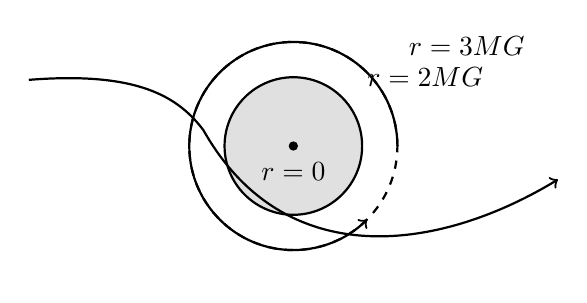
\begin{tikzpicture}[scale=1.12]
\fill[black!12] (0,0) circle (0.78);
\draw[thick] (0,0) circle (0.78);
\draw[dashed,thick] (0,0) circle (1.18);
\fill (0,0) circle (1.5pt);
\draw[->,thick] (1.18,0) arc (0:315:1.18);
\draw[->,thick] (-3.0,0.75)
  .. controls (-1.75,0.85) and (-1.30,0.55) .. (-1.02,0.18)
  .. controls (-0.10,-1.45) and (1.65,-1.20) .. (3.0,-0.38);
\node[right] at (0.73,0.78) {\(r=2MG\)};
\node[right] at (1.20,1.13) {\(r=3MG\)};
\node[below] at (0,-0.08) {\(r=0\)};
\end{tikzpicture}
\caption{L’horizon, la sphère des photons et un rayon fortement dévié. Des rayons arbitrairement proches de l’orbite circulaire instable peuvent subir une déviation arbitrairement grande avant de s’échapper ou de tomber vers l’intérieur.}
\end{figure}

\begin{classroomqa}
\audiencequestion{Pourquoi maintenir le moment cinétique constant, et quel est son lien avec la fréquence d’un photon et sa trajectoire incidente ?}
\lecturerresponse{Chaque rayon porte un moment cinétique conservé par rapport au trou noir. Sa fréquence fixe la norme de sa quantité de mouvement, tandis que son décalage par rapport au centre contribue à déterminer \(L\). En dehors d’une orbite circulaire, le rayon et le moment cinétique peuvent être choisis indépendamment. La condition d’orbite circulaire lie le mouvement au rayon unique \(3MG\), et la factorisation de l’équation ~\eqref{eq:l6-photon-energy} montre que ce rayon est indépendant de la valeur de \(L\).
\lecturetimestamp{00:54:43--00:57:02}}
\end{classroomqa}

\begin{classroomqa}
\audiencequestion{Pourquoi le maximum de l’énergie permet-il de repérer une orbite ?}
\lecturerresponse{Une fois le mouvement angulaire éliminé à \(L\) fixé, la fonction restante joue le rôle d’une énergie radiale effective. Un point stationnaire assure l’équilibre radial. Un minimum serait stable ; ce point est un maximum, et correspond donc à une orbite circulaire instable. Il n’y a aucune contradiction à parler à la fois d’équilibre et d’instabilité.
\lecturetimestamp{00:57:51--00:58:54}}
\end{classroomqa}

Une particule massive peut suivre des orbites circulaires de genre temps à l’extérieur de \(3MG\), mais celles qui se trouvent le plus près de la sphère des photons sont instables. Une particule sans masse ne possède qu’une seule orbite circulaire, à \(3MG\). À l’intérieur de la sphère des photons, un photon en mouvement tangentiel tombe vers l’intérieur ; un objet plus lent n’a pas davantage de chances de maintenir une telle orbite. Cette affirmation concerne le mouvement angulaire. À l’extérieur de l’horizon, un rayon suffisamment dirigé vers l’extérieur peut encore s’échapper, même si son rayon initial est inférieur à \(3MG\).

\section{L’effet d’un trou noir sur une image}

La sphère des photons explique pourquoi un trou noir ne se réduit pas à un disque sombre plaqué sur un ciel par ailleurs inchangé. La lumière provenant d’un objet d’arrière-plan peut parvenir à l’observateur par plusieurs chemins. Un rayon peut passer d’un côté du trou noir, un autre de l’autre côté, et d’autres encore peuvent en faire un ou plusieurs tours. L’image peut alors présenter des images décalées ou dédoublées, des anneaux et une suite infinie d’images toujours plus fines et plus faibles, associées aux tours supplémentaires. L’image exacte est complexe, mais son origine est déjà contenue dans l’orbite instable.

Lorsque la source, la lentille et l’observateur sont suffisamment alignés, l’image peut former un anneau d’Einstein. On observe des anneaux dus à la lentille gravitationnelle dans la nature. Pour obtenir l’image complète du trou noir, il faut intégrer les géodésiques de genre lumière pour de nombreuses directions initiales ; c’est un calcul qui se prête bien à l’ordinateur.

\begin{classroomqa}
\audiencequestion{Cette limite optique désigne-t-elle la sphère des photons ou l’horizon ?}
\lecturerresponse{Ces deux surfaces jouent des rôles différents. L’horizon en \(2MG\) est la limite causale : aucun signal dirigé vers le futur ne s’échappe de son intérieur. La sphère des photons en \(3MG\) régit le mouvement tangentiel et la forte lentille gravitationnelle. Entre les deux rayons, un rayon radial dirigé vers l’extérieur peut s’échapper, tandis qu’un rayon tangent tombe vers l’intérieur. Des directions intermédiaires peuvent donner lieu à des boucles avant l’évasion ou la capture.
\lecturetimestamp{01:02:47--01:03:40}}
\end{classroomqa}

\begin{classroomqa}
\audiencequestion{Peut-on calculer un trajet lumineux quelconque au lieu de se contenter de l’esquisser ?}
\lecturerresponse{Oui. Il suffit d’introduire la condition de nullité dans les équations géodésiques ou d’Euler--Lagrange, puis d’intégrer avec les données initiales choisies. Les équations ne présentent rien de conceptuellement nouveau, mais le calcul de trajectoire des rayons est algébriquement fastidieux ; c’est pourquoi le calcul numérique est la méthode pratique pour construire une image.
\lecturetimestamp{01:03:48--01:04:27}}
\end{classroomqa}

\begin{classroomqa}
\audiencequestion{L’application directe des équations d’Euler--Lagrange aurait-elle compliqué le calcul des orbites circulaires ?}
\lecturerresponse{Elle aurait donné le même résultat. Dans les deux méthodes, l’action est le bon point de départ, mais les coordonnées cycliques font apparaître l’énergie et le moment cinétique conservés. Utiliser d’abord ces constantes est le chemin le plus court vers la condition d’orbite circulaire.
\lecturetimestamp{01:04:33--01:05:49}}
\end{classroomqa}

\section{La métrique au voisinage de l’horizon est celle de l’espace de Rindler}

Revenons maintenant à l’horizon. Les coefficients de Schwarzschild semblent y diverger ou s’annuler, et leurs signes s’échangent lors du franchissement de l’horizon. Pourtant, un observateur en chute ne rencontre à cette surface aucune courbure locale divergente. Le principe d’équivalence nous indique comment ces deux affirmations peuvent être vraies à la fois.

Partons de l’espace-temps de Minkowski en deux dimensions :
\begin{equation}
d\tau^{2}=dT^{2}-dX^{2}.
\end{equation}
Dans le secteur droit de Rindler, définissons
\begin{equation}
X=\rho\cosh\omega,
\qquad
T=\rho\sinh\omega.
\label{eq:l6-rindler-map}
\end{equation}
Les courbes à \(\rho\) constant vérifient
\begin{equation}
X^{2}-T^{2}=\rho^{2},
\end{equation}
Ce sont donc des hyperboles, correspondant aux lignes d’univers d’observateurs uniformément accélérés. En substituant l’équation ~\eqref{eq:l6-rindler-map} dans la métrique plate, on obtient
\begin{equation}
d\tau^{2}
=\rho^{2}d\omega^{2}-d\rho^{2}.
\label{eq:l6-rindler-metric}
\end{equation}
Posons maintenant
\begin{equation}
\rho^{2}=4\xi,
\qquad
\omega=\frac{t}{2}.
\label{eq:l6-rindler-rescale}
\end{equation}
Puisque \(d\rho^{2}=d\xi^{2}/\xi\), l’équation ~\eqref{eq:l6-rindler-metric} devient
\begin{equation}
d\tau^{2}
=\xi\,dt^{2}-\frac{d\xi^{2}}{\xi}.
\label{eq:l6-xi-metric}
\end{equation}

\begin{classroomqa}
\audiencequestion{Où sont passées les coordonnées angulaires ou transverses ?}
\lecturerresponse{Nous les avons simplement omises. Nous étudions le plan local \(t\)-\(r\) où se manifeste le comportement au franchissement de l’horizon. Les deux directions transverses restent régulières et peuvent être réintroduites ; elles ne changent pas la singularité de coordonnées que nous analysons.
\lecturetimestamp{01:16:27--01:16:47}}
\end{classroomqa}

Pour comparer avec Schwarzschild, choisissons des unités telles que \(2MG=1\). La partie radiale de l’équation ~\eqref{eq:l6-schwarzschild} est
\begin{equation}
d\tau^{2}
=
\frac{r-1}{r}\,dt^{2}
-
\frac{r}{r-1}\,dr^{2}.
\end{equation}
Tout près de \(r=1\), il faut conserver le petit numérateur \(r-1\), tandis que les facteurs \(r\), autrement sans effet notable, peuvent être remplacés par un. Ainsi,
\begin{equation}
d\tau^{2}
\simeq
(r-1)\,dt^{2}
-
\frac{dr^{2}}{r-1}.
\end{equation}
Avec
\begin{equation}
\xi=r-1,
\end{equation}
on retrouve exactement l’équation ~\eqref{eq:l6-xi-metric}. Au voisinage de l’horizon, la géométrie de Schwarzschild est localement décrite par l’espace-temps plat en coordonnées de Rindler.

\begin{classroomqa}
\audiencequestion{Comment ces coordonnées peuvent-elles être accélérées si l’espace-temps sous-jacent est plat ?}
\lecturerresponse{L’accélération est une propriété de l’observateur, pas nécessairement de la courbure. Dans l’espace-temps de Minkowski, une ligne d’univers à \(\rho\) constant est uniformément accélérée. De même, un observateur maintenu à rayon fixe près d’un trou noir doit être soutenu pour résister à la chute libre. Le principe d’équivalence rend les descriptions locales compatibles, même si l’espace-temps de Schwarzschild dans son ensemble est courbe.
\lecturetimestamp{01:22:19--01:24:06}}
\end{classroomqa}

\section{Franchir l’horizon de Rindler}

Les formules du secteur droit ne couvrent que \(\xi>0\) :
\begin{equation}
X=2\sqrt{\xi}\cosh\frac{t}{2},
\qquad
T=2\sqrt{\xi}\sinh\frac{t}{2}.
\label{eq:l6-rindler-outside}
\end{equation}
La surface \(\xi=0\) est la droite nulle \(X=T\). Pour poursuivre dans le secteur futur, posons
\begin{equation}
\zeta=-\xi>0
\end{equation}
et échangeons les rôles des fonctions hyperboliques :
\begin{equation}
T=2\sqrt{\zeta}\cosh\frac{t}{2},
\qquad
X=2\sqrt{\zeta}\sinh\frac{t}{2}.
\label{eq:l6-rindler-inside}
\end{equation}
La métrique reste
\begin{equation}
d\tau^{2}
=\xi\,dt^{2}-\frac{d\xi^{2}}{\xi},
\end{equation}
mais lorsque \(\xi<0\), le coefficient de \(dt^{2}\) est négatif et celui de \(d\xi^{2}\) est positif. La coordonnée \(\xi\), et donc la direction radiale de Schwarzschild, est devenue de genre temps ; \(t\) est devenue de genre espace.

\begin{figure}[htbp]
\centering
\includegraphics[width=0.88\textwidth]{lecture_06_figure_06.png}
\caption{Les secteurs de Rindler, leurs frontières nulles et le prolongement de \(\xi>0\) vers \(\xi<0\). Le tableau indique également \(\rho^{2}=4\xi\) et \(\omega=t/2\).}
\lectureframe{01:29:40}
\end{figure}

\begin{classroomqa}
\audiencequestion{Certaines courbes de ce diagramme de coordonnées se déplacent-elles plus vite que la lumière ?}
\lecturerresponse{Une ligne du quadrillage des coordonnées n’est pas nécessairement la ligne d’univers d’un objet matériel. Sa pente dans les coordonnées peut sembler supraluminique sans qu’il y ait violation de la causalité. Les rayons lumineux physiques restent sur les lignes nulles, et les particules physiques restent à l’intérieur de leurs cônes de lumière locaux.
\lecturetimestamp{01:28:44--01:29:08}}
\end{classroomqa}

En poursuivant plus loin dans l’intérieur de Schwarzschild, on finit par atteindre \(r=0\). Cette frontière est de genre espace. Il vaut donc mieux la décrire comme un temps que comme un lieu : toute trajectoire de genre temps ou nulle, dirigée vers le futur dans l’intérieur du trou noir, l’atteint. On peut contourner un lieu. On ne peut pas contourner son propre futur.

\begin{classroomqa}
\audiencequestion{Le diagramme peut-il simplement se prolonger au-delà de \(r=0\) jusqu’aux valeurs négatives de \(r\), et \(r=0\) correspond-il toujours au centre ?}
\lecturerresponse{Le dessin des coordonnées peut inciter à prolonger une ligne, mais la solution classique de Schwarzschild s’arrête à la singularité de courbure. On peut toujours appeler \(r=0\) le centre, mais c’est un centre très inhabituel : à l’intérieur, c’est une frontière future de genre espace. Il n’existe pas de passage régulier à travers elle vers une région de rayon négatif.
\lecturetimestamp{01:32:16--01:34:06}}
\end{classroomqa}

\begin{classroomqa}
\audiencequestion{Les axes diagonaux du diagramme de Rindler sont-ils de genre lumière, et un observateur en chute peut-il y entrer à une valeur finie du temps accéléré ?}
\lecturerresponse{Oui, les frontières du secteur sont des droites nulles. Une ligne d’univers en chute libre traverse une telle droite en un événement ordinaire, au bout d’un temps propre fini. La coordonnée accélérée \(t\), ou de façon équivalente \(\omega\), n’est pas bornée le long de la description extérieure à \(\rho\) constant ; c’est cette attribution de coordonnées, et non l’événement du franchissement, qui devient infinie.
\lecturetimestamp{01:34:26--01:35:03}}
\end{classroomqa}

\section{Alice à l’extérieur et Bob en chute libre}

Supposons qu’Alice reste à l’extérieur, à rayon fixe, soutenue contre la gravité, tandis que Bob chute librement. Près de l’horizon, Alice suit une hyperbole analogue à celle de Rindler. Ses tranches à \(t\) constant se resserrent de plus en plus près de la frontière nulle. Tout événement de la ligne d’univers de Bob auquel Alice attribue une valeur finie de \(t\) se trouve à l’extérieur de l’horizon ; elle n’attribue donc jamais un temps de Schwarzschild fini au franchissement de Bob.

Bob emporte une horloge mesurant le temps propre. Sa trajectoire traverse la ligne nulle pendant un intervalle fini sur cette horloge. Rien de localement divergent ne se produit lors du franchissement. L’horizon est déterminant à l’échelle globale, mais localement ordinaire.

\begin{figure}[htbp]
\centering
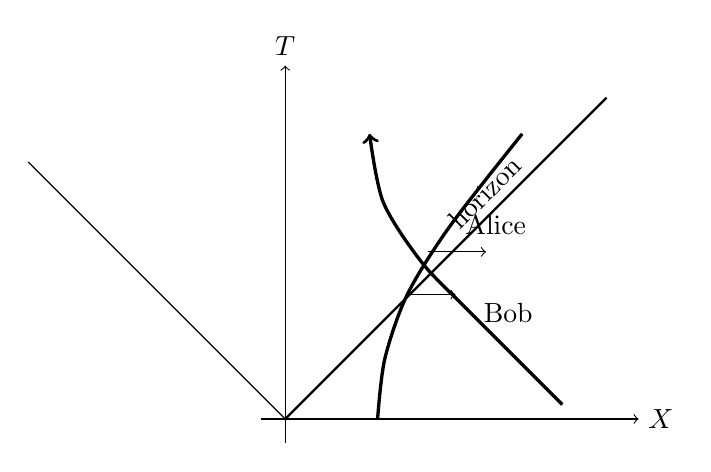
\begin{tikzpicture}[scale=1.02]
\draw[->] (-0.3,0) -- (4.4,0) node[right] {\(X\)};
\draw[->] (0,-0.3) -- (0,4.4) node[above] {\(T\)};
\draw[thick] (0,0) -- (4.0,4.0);
\draw[thin] (0,0) -- (-3.2,3.2);
\node[rotate=45,above] at (2.65,2.65) {horizon};
\draw[very thick]
  plot[smooth] coordinates {(1.15,0.0) (1.24,0.75) (1.52,1.55)
  (2.05,2.40) (2.95,3.55)};
\node[right] at (2.12,2.42) {Alice};
\draw[very thick,->]
  plot[smooth] coordinates {(3.45,0.18) (2.85,0.78) (2.25,1.38)
  (1.70,1.95) (1.22,2.70) (1.05,3.55)};
\node[right] at (2.35,1.32) {Bob};
\draw[->] (1.52,1.55) -- (2.12,1.55);
\draw[->] (1.78,2.08) -- (2.50,2.08);
\end{tikzpicture}
\caption{La ligne d’univers accélérée d’Alice à l’extérieur et celle de Bob en chute libre. Les tranches de coordonnées d’Alice s’approchent de l’horizon ; Bob le franchit en un temps propre fini.}
\end{figure}

\begin{classroomqa}
\audiencequestion{Que voit Bob lorsqu’il regarde Alice, et que devient son horloge après le franchissement ?}
\lecturerresponse{Bob voit Alice s’éloigner en accélérant comme il le faut pour rester à l’extérieur, mais il ne voit aucun événement singulier lors de son franchissement. Alice peut être maintenue à rayon fixe ; l’orbite est une autre configuration possible. L’horloge de Bob continue normalement à mesurer son temps propre \(\tau\). À l’intérieur, dire que la coordonnée radiale est de genre temps décrit la géométrie causale ; cela ne transforme pas littéralement sa montre-bracelet en règle graduée. Sa ligne d’univers prend finalement fin en \(r=0\).
\lecturetimestamp{01:39:51--01:44:45}}
\end{classroomqa}

Nous comprenons maintenant que la ligne nulle est l’horizon lui-même, et non simplement un point où un coefficient de coordonnées se comporte mal. À l’extérieur, une famille de rayons lumineux radiaux se dirige vers l’extérieur. À l’intérieur, les deux directions futures du cône de lumière mènent vers des valeurs décroissantes de \(r\). Toute trajectoire future massive doit rester entre ces deux directions nulles et atteint donc la singularité.

\section{Signaux, décalage vers le rouge et formation d’un horizon}

Supposons que la matière en effondrement émette une suite régulière d’impulsions lumineuses. Un observateur lointain reçoit les impulsions successives à des intervalles de plus en plus longs. Leurs fréquences se décalent de l’optique vers l’infrarouge, les micro-ondes, les ondes radio, puis vers des longueurs d’onde encore plus grandes. Dans un calcul classique idéalisé, l’observateur extérieur peut continuer à associer des signaux toujours plus tardifs à la matière qui s’approche de l’horizon, mais la source devient rapidement trop rouge et trop faible pour être détectée en pratique.

\begin{classroomqa}
\audiencequestion{Pendant l’effondrement, un observateur extérieur voit-il simplement toute la matière se figer à l’horizon ?}
\lecturerresponse{En temps de Schwarzschild, la surface de la matière en effondrement s’approche asymptotiquement de l’horizon et semble se figer de plus en plus. Ce qui est effectivement observé est codé dans les signaux lumineux, qui arrivent de plus en plus tard, sont de plus en plus décalés vers le rouge et s’affaiblissent. Cette description en coordonnées n’implique pas que la matière en chute subisse un temps propre infini.
\lecturetimestamp{01:47:06--01:48:11}}
\end{classroomqa}

\begin{classroomqa}
\audiencequestion{Un observateur suffisamment patient pourrait-il reconstituer toute l’histoire de la chute ?}
\lecturerresponse{Uniquement à partir des signaux émis qui parviennent jusqu’à lui. Les impulsions successives sont de plus en plus espacées et décalées vers le rouge. Un observateur idéal, doté d’une sensibilité illimitée, pourrait suivre le signal classique jusqu’à des longueurs d’onde toujours plus grandes ; un observateur réel voit l’objet s’effacer.
\lecturetimestamp{01:48:13--01:52:00}}
\end{classroomqa}

\begin{classroomqa}
\audiencequestion{Que signifie exactement l’affirmation selon laquelle la singularité est un temps plutôt qu’un lieu ?}
\lecturerresponse{La surface \(r=0\) est de genre espace. Une fois à l’intérieur de l’horizon, toute courbe de genre temps ou nulle dirigée vers le futur s’y termine. On peut éviter un lieu en empruntant un autre chemin dans l’espace ; on ne peut éviter une frontière future tout en suivant une ligne d’univers dirigée vers le futur.
\lecturetimestamp{01:52:02--01:53:10}}
\end{classroomqa}

Comment, alors, un trou noir peut-il se former ou augmenter sa masse si l’observateur extérieur ne voit jamais la matière le franchir ? Considérons une coquille sphérique en effondrement. L’horizon global n’attend pas comme une surface matérielle préexistante à un rayon fixe. Il apparaît au centre et s’étend vers l’extérieur, jusqu’à rejoindre la coquille au moment où la région du trou noir se forme. La description de Schwarzschild à l’extérieur montre néanmoins la coquille s’approcher asymptotiquement de l’horizon final. La représentation complète de l’espace-temps, y compris la détermination globale de la position de l’horizon, sera le sujet du prochain cours.

\begin{figure}[htbp]
\centering
\includegraphics[width=0.90\textwidth]{lecture_06_figure_07.png}
\caption{Une coquille en effondrement et l’horizon, qui s’étend depuis le centre vers l’extérieur jusqu’à sa rencontre avec la coquille. Ce dessin annonce la géométrie globale de l’effondrement qui sera développée au prochain cours.}
\lectureframe{01:57:25}
\end{figure}

\begin{classroomqa}
\audiencequestion{Si rien ne franchit l’horizon en temps coordonné extérieur, comment un trou noir peut-il se former ou grandir ?}
\lecturerresponse{La prémisse mêle une affirmation sur les coordonnées et une affirmation globale. La matière en effondrement atteint la région concernée en un temps propre fini, tandis que l’horizon des événements est déterminé par la structure causale de tout l’espace-temps. Dans le modèle de la coquille, il apparaît au centre et s’étend vers l’extérieur jusqu’à rejoindre la coquille. La vision retardée et décalée vers le rouge de l’observateur extérieur reste compatible avec cet horizon global.
\lecturetimestamp{01:53:11--01:57:34}}
\end{classroomqa}

\section{Les directions d’échappement entre les deux sphères}

L’horizon et la sphère des photons répartissent les trajectoires lumineuses en différents cas. À un rayon
\begin{equation}
2MG<r<3MG,
\end{equation}
un rayon lumineux radial dirigé vers l’extérieur peut s’échapper à l’infini. Un rayon lumineux tangent ne le peut pas ; il tombe vers l’intérieur. Entre ces deux directions se trouve un cône d’échappement. À mesure que l’on s’approche de l’horizon, ce cône se resserre autour de la direction radiale vers l’extérieur. Une fois l’horizon franchi, il se referme complètement.

\begin{classroomqa}
\audiencequestion{Une source lumineuse située entre l’horizon et la sphère des photons peut-elle émettre un signal vers l’extérieur ?}
\lecturerresponse{Oui. Un rayon nul dirigé suffisamment près de la direction radiale vers l’extérieur s’échappe tant que son événement d’émission se situe à l’extérieur de \(2MG\). Dire que le mouvement angulaire à l’intérieur de \(3MG\) mène vers l’intérieur n’interdit pas une échappée radiale. L’issue dépend de la direction d’émission, et le cône vers l’extérieur admissible se resserre à mesure que la source s’approche de l’horizon.
\lecturetimestamp{01:57:34--01:59:48}}
\end{classroomqa}

\begin{classroomqa}
\audiencequestion{Un rayon arrivant de l’extérieur peut-il pénétrer à l’intérieur de la sphère des photons, faire demi-tour et ressortir ?}
\lecturerresponse{Pas le long d’une géodésique nulle du type considéré. Au point de rebroussement, la vitesse radiale serait nulle : le rayon serait donc momentanément tangent à un rayon inférieur à \(3MG\) ; à cet endroit, la trajectoire angulaire mène vers l’intérieur au lieu de repartir vers l’extérieur. Une source déjà située entre les deux sphères peut néanmoins émettre un rayon dirigé suffisamment près de la direction radiale vers l’extérieur avant de franchir l’horizon.
\lecturetimestamp{01:59:49--02:01:27}}
\end{classroomqa}

La dernière question est volontairement moins tranchée. Imaginons Alice et Bob maintenus tous deux au même rayon, à l’extérieur de l’horizon. Des observateurs proches peuvent manifestement échanger des signaux. S’ils sont très éloignés l’un de l’autre sur la sphère, le trajet nul direct et sa portée angulaire limite nécessitent un calcul géodésique explicite. La classe propose un itinéraire indirect : envoyer le message presque radialement vers l’extérieur jusqu’à un relais situé à un rayon plus sûr, le faire acheminer autour du trou noir à cet endroit, puis le renvoyer vers l’intérieur. Une autre possibilité consiste à lancer vers l’extérieur un objet ou un signal qui fait demi-tour et revient. Ces itinéraires montrent que l’impossibilité d’une orbite circulaire tangentielle n’interdit pas, à elle seule, toute communication entre observateurs extérieurs.

\begin{classroomqa}
\audiencequestion{Deux observateurs maintenus au même rayon, près de l’horizon, peuvent-ils communiquer autour du trou noir ?}
\lecturerresponse{Localement, oui. Pour des observateurs très éloignés ou diamétralement opposés, la limite du trajet direct n’a pas été établie dans le cours et ne doit pas être présentée comme un théorème. La discussion laisse d’abord ouverte cette question de géodésique angulaire, puis remarque qu’un signal indirect peut être envoyé presque radialement vers l’extérieur, relayé à un rayon plus grand, puis renvoyé. À mesure qu’on s’approche de l’horizon, la portée angulaire directement exploitable se rétrécit de plus en plus, mais une voie vers l’extérieur reste possible tant qu’on se trouve hors de l’horizon.
\lecturetimestamp{02:01:29--02:04:17}}
\end{classroomqa}

L’étape suivante consiste à remplacer ces esquisses près de l’horizon par la géométrie globale d’un corps en effondrement et à examiner précisément comment un horizon des événements se forme et s’étend.